\documentclass{article}
\usepackage[utf8]{inputenc}

% ---------------ShareLatex Hotkeys------------
% Select + TAB  - ->         indents
% Select + SHIFT + TAB - ->  un-indents
% CTRL + ENTER - ->          Recompiles


% Use wide margins, but not quite so wide as fullpage.sty
\marginparwidth 0.5in 
\oddsidemargin 0.15in 
\evensidemargin 0.15in 
\marginparsep 0.25in
\topmargin 0.15in 
\textwidth 6.5in \textheight 8 in
\hbadness=10000			% No "underfull hbox" messages.
% That's about enough definitions

\usepackage{amsmath, amssymb}
\usepackage{latexsym}
\usepackage[utf8]{inputenc}
\usepackage{xcolor}
\usepackage{url}
\usepackage{graphicx}
\graphicspath{ {images/} }


%===================================================================
% Macros.
%===================================================================
\newcommand{\problem}[1]{\section{#1}}		% Problem.
\newcommand{\new}[1]{{\em #1\/}}		    % New term (set in italics).
\newcommand{\set}[1]{\{#1\}}			    % Set (as in \set{1,2,3})
\newcommand{\setof}[2]{\{\,{#1}|~{#2}\,\}}	% Set ( as in \setof{x}{x > 0} )
\newcommand{\C}{\mathbb{C}}	                % Complex numbers.
\newcommand{\N}{\mathbb{N}}                 % Positive integers.
\newcommand{\Q}{\mathbb{Q}}                 % Rationals.
\newcommand{\R}{\mathbb{R}}                 % Reals.
\newcommand{\Z}{\mathbb{Z}}                 % Integers.
\newcommand{\compl}[1]{\overline{#1}}		% Complement of ...
\newcommand{\powerset}[1]{\mathcal{P}(#1)}

\newcommand{\rd}[1]{\textcolor{red}{#1}}
\newcommand{\bl}[1]{\textcolor{blue}{#1}}
\newcommand{\gr}[1]{\textcolor{green}{#1}}





\title{Network Science--A Brief Overview}
\author{Natalie Nagata \\ Dr. William DeMeo \\ University of Hawai\textquoteleft i at M\=anoa}
\date{\today}

\begin{document}

\maketitle

\section{Introduction}
Science and technology has advanced at ever increasing rates over the past few decades.  As a result, the study of complex networks has become a field of huge interest for having wide-ranging potential and applicability.  By using modern graph theory, we can analyze the structure of networks to understand characteristics that weren't previously well understood. We shall provide a brief discussion of some different models ised in network analysis and their applications.  This paper is not meant to be comprehensive but aims to provide a short overview for readers who are new to network science. But first, before discussing some basic models in network science, it is helpful to go over some basic concepts in graph theory.  



%%%%%%%%%%%%%%%%%%%%%%%%%%%%%%%%%%%%%%%%%%%%%%%%%%%
\section{Basics}

The fundamentals of network science are based in graph theory.  A graph $G=(V,E)$ is defined as an ordered pair which consists of a nonempty set of vertices $V$ and a set of edges $E$.  

For the remainder of this paper, we shall denote the number of vertices as $N = |V|$ and the number of edges as $L= |E|$. Each vertex can be labeled such that $V = \{ v_1 , v_2 , \ldots , v_N\}$ and, similarly, each edge can be labeled such that $E = \{e_1 , e_2 , \ldots , e_L  \}$. Each edge must be connected to one or two vertices (sometimes called \textit{endpoints} \; \cite{discrete}). Thus each edge may be represented as  Visually, you may think of graphs/networks as a diagram that consists of points (vertices) and there may be lines (edges) connected between two points which represent relationships between two points. (See Fig \ref{fig:graph} )  Note that graph and network theorists essentially study the same systems but describe them within their respective fields using different terminology.  Graph theorists tend to consider ``vertices'' and ``edges'' whereas network theorists study ``nodes'' and ``links'.'  All of these terms shall be used interchangeably from here on (although the symbolic representation shall remain as mentioned previously).


% ----Fig: simple/multi graph----
\begin{figure}[h]
    \center
    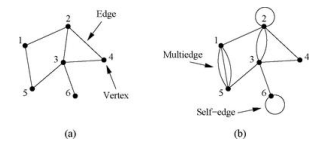
\includegraphics[scale=1.0]{newman-graphs}
    \caption{(a) a simple undirected graph, (b) an undirected graph with multiedges and loops.   \cite{newman}}
    \label{fig:graph}
\end{figure}


% -----subsection--------
\subsection{Types of Graphs}
Graphs and networks are categorized in a variety of ways. A \textit{simple graph} is a graph such that there exists at most only one edge between any pair of vertices and does not contain any looped edges (edges that begin and end at the same vertex).  Note that a graph does not necessarily contain edges. Nodes that have no adjacent edges are referred to as \textit{isolates}.  Graphs that are not simple are known as \textit{multigraphs} since they may contain multiple links between the same pair of vertices.  Multigraphs may also contain loops. (See Fig. \ref{fig:graph})

% ----Fig: directed graph----
\begin{figure}[h]
    \center
    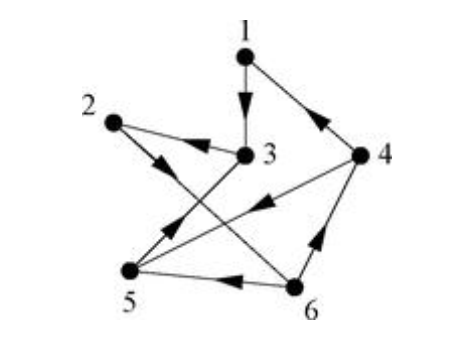
\includegraphics[scale=0.6]{newman-directed}
    \caption{a directed graph with arrows representing the direction of edges  \cite{newman}}
    \label{fig:digraph}
\end{figure}


Another distinguishing property is whether a network is directed or undirected.  An \textit{undirected} network contains edges that have no defined ``direction'' associated with it. So an edge with endpoints $v_a$ and $v_b$ is the same as an edge with endpoints $v_b$ and $v_a$.  A \textit{directed} network has edges with an ordered pair of vertices as endpoints.  (See Fig. \ref{fig:digraph})


% -----subsection--------
\subsection{Representation}
As we've seen before, graphs can be visually drawn as a collection of vertices connected by edges (see Fig. \ref{fig:graph}).  But how do we objectively quantify the relationships a system has between nodes and edges?  

Often we can represent a graph numerically with what's known as an \textit{adjacency matrix}. Consider an adjacency matrix $\textbf{A}$.  For a simple undirected graph, the entries $a_{ij}$ of its adjacency matrix $\textbf{A}$ are such that 


\begin{equation}
 \textbf{A} =
\begin{cases}
1 & \text{if an edge exists between $v_i$ and $v_j$},\\
0 & \text{otherwise}.
\end{cases}
\end{equation}

\vspace{0.4cm}

For example, the adjacency matrices for Fig. \ref{fig:graph}(a) and Fig. \ref{fig:graph}(b) are 

\begin{equation}
\textbf{A} =
    \begin{bmatrix}
    0 & 1 & 0 & 0 & 1 & 0 \\
    1 & 0 & 1 & 1 & 0 & 0 \\
    0 & 1 & 0 & 1 & 1 & 1 \\
    0 & 1 & 1 & 0 & 0 & 0 \\
    1 & 0 & 1 & 0 & 0 & 0 \\
    0 & 0 & 1 & 0 & 0 & 0 
    \end{bmatrix}
\end{equation}

\begin{equation}
\textbf{A} =
    \begin{bmatrix}
    0 & 1 & 0 & 0 & 3 & 0 \\
    1 & 2 & 2 & 1 & 0 & 0 \\
    0 & 2 & 0 & 1 & 1 & 1 \\
    0 & 1 & 1 & 0 & 0 & 0 \\
    3 & 0 & 1 & 0 & 0 & 0 \\
    0 & 0 & 1 & 0 & 0 & 2 
    \end{bmatrix}
\end{equation}

\vspace{0.4cm}

For directed networks, their adjacency matrices are based on a similar idea as previously described.  The main difference is that the row and column that each entry belongs to corresponds to  the beginning and endpoint of each edge. Thus,

\begin{equation}
\textbf{A}_{ij} =
\begin{cases}
1 & \text{if an edge exists \textit{from} $v_j$ \textit{to} $v_i$},\\
0 & \text{otherwise}.
\end{cases}
\end{equation}

\vspace{0.4cm}

Thus, the adjacency matrix for the directed network in Fig. \ref{fig:digraph} is

\begin{equation}
\textbf{A} =
    \begin{bmatrix}
    0 & 0 & 0 & 1 & 0 & 0 \\
    0 & 0 & 1 & 0 & 0 & 0 \\
    1 & 0 & 0 & 0 & 1 & 0 \\
    0 & 0 & 0 & 0 & 0 & 1 \\
    0 & 0 & 0 & 1 & 0 & 1 \\
    0 & 1 & 0 & 0 & 0 & 0 
    \end{bmatrix}
\end{equation}





% -----subsection--------
\subsection{Measurements}

There are different properties of graphs which we can numerically measure as well.  For undirected netowkrs, the number of edges that each vertex $v_i$ is adjacent to is called the \textit{degree} of $v_i$ and is denoted as $k_i$. Thus, the total number of links $L$ of a network is 

\begin{equation}
L = \frac{1}{2} \sum_{i=1}^{N} k_i
\end{equation}

For directed networks, we need to make the distinction between edges that point towards a vertex versus edges that point away from a vertex. For each vertex $v_i$, there is a corresponding \textit{in-degree} and \textit{out-degree} value, $k_i^{in}$ and $k_i^{out}$, that represent the number of edges pointing inwards to $v_i$ and outwards to $v_i$, respectively.

\begin{equation}
k_i = k_i^{in} + k_i^{out}
\end{equation}

The average degree of a network is defined as the sum of the degrees of each vertex divided by $N$. As such, for any graph $G$, its average degree is

\begin{equation}\label{eq:avgdegreedirect}
avg(k) = \frac{1}{N} \sum_{i=1}^N k_i = \frac{2L}{N}
\end{equation}

For directed graphs the definition differs slightly to account for in- and out-degree distinction.  The total number of links $L$ is 

\begin{equation}\label{eq:totaldegreedirect}
L = \sum_{i=1}^N k_i^{in} = \sum_{i=1}^N k_i^{out}
\end{equation}


From Eqn. \ref{eq:avgdegreedirect} and \ref{eq:totaldegreedirect}, it follows that

\begin{equation}
avg(k) = \frac{1}{N} \sum_{i=1}^N k_i^{in} = \frac{1}{N}\sum_{i=1}^N =  k_i^{out} = \frac{L}{N}
\end{equation}



In addition to average degree, the degree distribution of a network is a very measurement in network science.  The \textit{degree distribution} of a network describes the probability $p_k$ that a randomly selected node is of degree $k$, where $\sum_{i=0}^{\infty} p_k = 1$.  An example of the degree distribution representation network is provided below.



% ------FIG degree distribution-----------
\begin{figure}[h]
    \center
    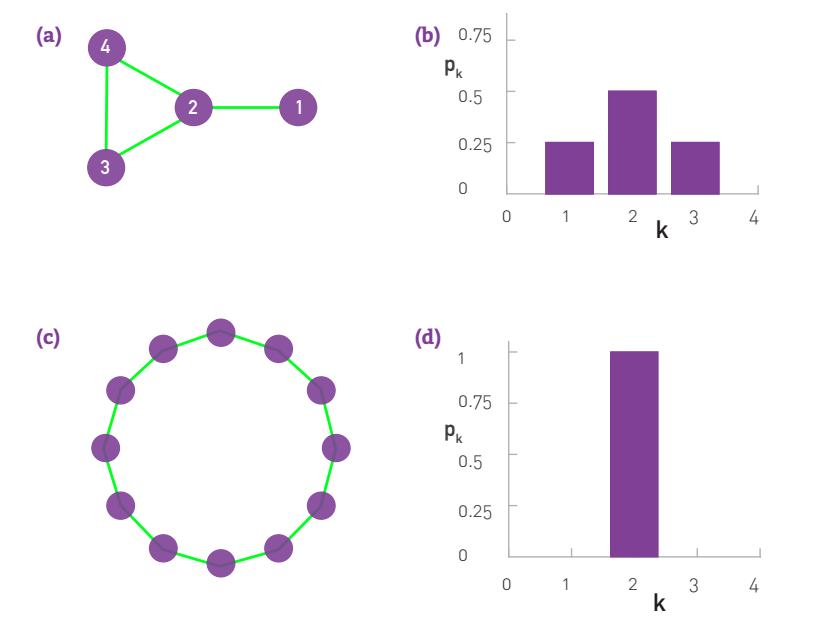
\includegraphics[scale=0.45]{ns-degdistribution}
    \caption{Two representations of the degree distribution of two small networks  \cite{ns}}
    \label{fig:degdistribution}
\end{figure}




Additionally, the concept of \textit{geodesic distance} (or just \textit{distance}) is important when studying networks.  This is analogous to the idea of paths in graph theory.  Informally, a \textit{path} is a sequence of $n$ vertices and $n-1$ edges that begin at vertex $v_1$ and end at some vertex $v_n$ \cite{discrete}. In network theory, the geodesic distance generally refers the shortest possible path between two vertices.  It is also possible for no geodesic distance to exist between two  vertices.  These vertices are disconnected from each other.  Usually they belong to different components within a network or one or both nodes are isolates.  In contrast, the \textit{diameter} of a network is the largest distance in a network, denoted as $d_{max}$.  We will see later how the distance, average degree, and diameter of a network are related.






%%%%%%%%%%%%%%%%%%%%%%%%%%%%%%%%%%%%%%%%%%%%%%%%%%%%%%
\section{Models}

\subsection{Random Graphs}

The overall motivation of network science  is to create and study models of real-world networks. These real-world networks differ from other systems such as a lattice.  The most striking differences are with a network's lack of repetitive and orderly structure like that of a lattice.  One of the earliest models is that of a \textit{random graph}.  It was first studied by Anatol Rapoport in 1951 but was brought to more well-known attention by P\' al Erd\H os and Alfr\' ed R\' enyi in 1959 \cite{ns}.  They are historically recognized as the founders of random graph theory by merging techniques from the fields of combinatorics, graph theory, and probability.  As a result, random graphs are generally called \textit{Erd\H os-R\' enyi graphs}.

There are two ways of defining random networks.  A graph that follows the \textit{G(N, L)} model depends on a fixed $N$ total number of nodes and $L$ total number of links.  In the $G(N,L)$ model, a collection of all possible configurations of graphs with $N$ nodes and randomly placed $L$ links is generated. As such, each unique graph has an equivalent chance of being selected from this collection. The graph selected from this collection is the graph that is constructed.

In contrast, the  \textit{G(N, p)} model depends on the $N$ total number of nodes and a fixed probability $p$ that an edge exists between each pair of nodes of a network.  Starting with a collection of $N$ isolates, a random number between 0 or 1 is generated for each  pair of nodes in the system.  Depending on whether the number falls above or below the probability $p$ is what determines whether a link connects each pair of nodes.


% ------FIG random networks-----------
\begin{figure}[h]
    \center
    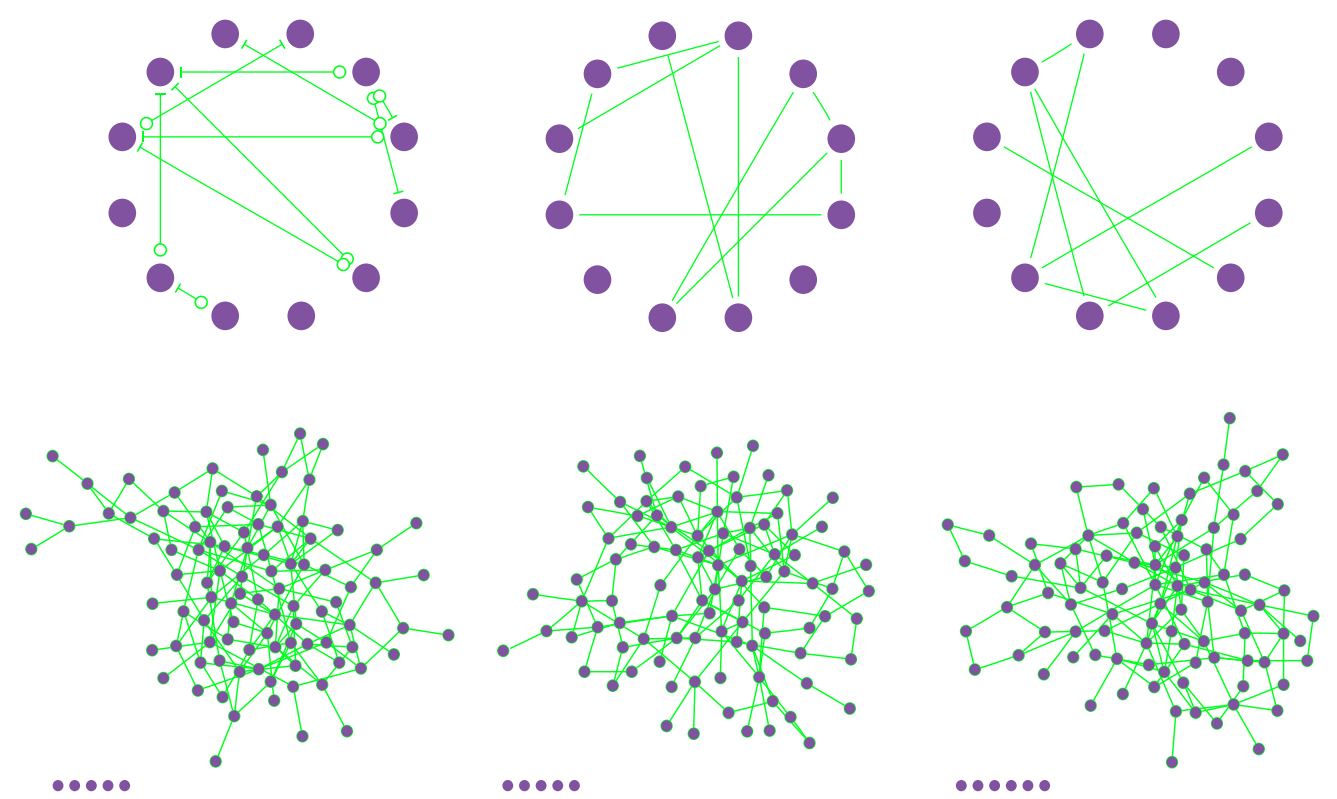
\includegraphics[scale=0.5]{ns-random}
    \caption{Three different representations of networks generated from the same $G(N,p)$ model with parameters $N=12$ and $p=\frac{1}{6}$  \cite{ns}}
    \label{fig:random}
\end{figure}



On average, random networks are predicted to consist of some nodes that have more links than others.  Since $p_k$ is the probability that a randomly chosen node is of degree $k$, the degree distribution of a network can be exactly described by the binomial distribution

% -------Eqn: BINOMIAL--------
\begin{equation}\label{eq:binomial}
    p_k = \binom{N-1}{k} p^k (1-p)^{N-k-1}
\end{equation}


As $N \rightarrow \infty$, the degree distribution can be approximated by the Poisson distribution

% --------Eqn: POISSON---------
\begin{equation}\label{eq:poisson}
    p_k = e^{- avg(k)} \frac{avg(k)^k}{k!}
\end{equation}

This behavior can be seen in Fig. \ref{fig:binompoisson}

\begin{figure}[h]
    \center
    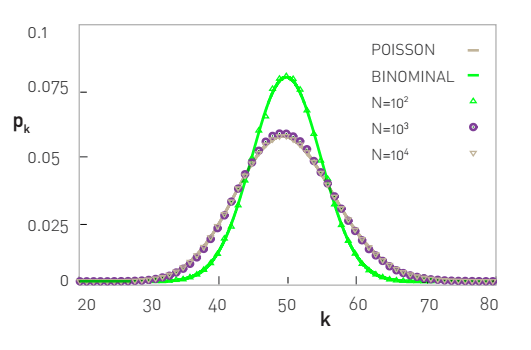
\includegraphics[scale=0.85]{ns-binomial}
    \caption{The degree distribution of three networks with $avg(k)=50$: a small network ($N=10^2$) which fits a binomial distribution (see Eq. \ref{eq:binomial}) in the green line, and large networks ($N = 10^3 \text{ and } N=10^4$ which approach the Poisson distribution (see Eq. \ref{eq:poisson}) in the gray line.  \cite{ns}}
    \label{fig:binompoisson}
\end{figure}

In more recent years,  technology has enabled us to effectively construct network maps of real-world systems.  This has led us to a surprising observation: real-world networks are not random. Barabasi highlights this by showing three examples of real-world networks and how their corresponding degree distributions deviate from their expected Poisson forms.


% -----FIG: REAL NETS-----------
\begin{figure}[h]
    \center
    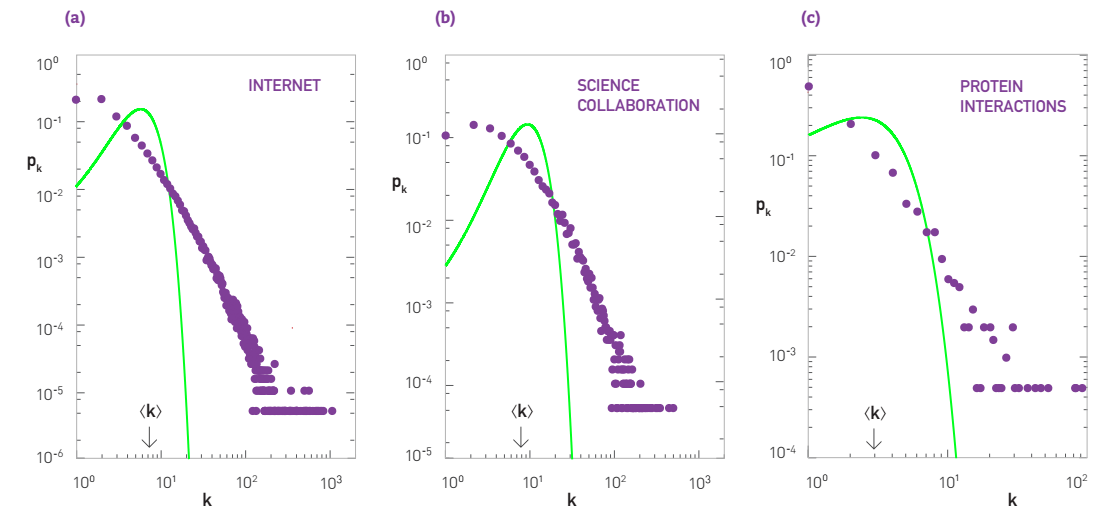
\includegraphics[scale=0.65]{ns-realnets}
    \caption{Plots of the degree distribution of three real networks (in purple) compared with their predicted Poisson degree distribution based on their measured average degree $k$. (a) Internet websites, (b) scientific collaborations based on PI's listed in published papers, (c) protein-protein interactions of biological systems \cite{ns}}
    \label{fig:realnets}
\end{figure}

What is the driving reason behind these differences?  Some of it can be explained by nodes that are of unusually high degree.  These high-degree nodes are known as \textit{hubs}. Hubs essentially dominate the characteristics of networks.  As we'll see in the next section, discussing hubs leads to an extension of the random network model called the Watts-Strogatz model.




% --------------------------------
% -------SMALL WORLD-------------
\subsection{Real-World Networks and the Small World Phenomenon}

The discrepancies between real-world systems and that of random-network models are revealed on closer inspection of our assumption that a Poisson distribution is the best fit.  The term $1 / k!$ in Eq. \ref{eq:poisson} results in greatly underestimating the number of hubs. Also the variance of nodes of average degree is much wider in real-world networks that that of random networks characterized by the Poisson distribution.  The presence of hubs leads to an idea known as the \textit{small world phenomenon}.  This is more widely known as \textit{six degrees of separation}.

The small world phenomenon stems from the Watts-Strogatz model which was proposed around 1998 \cite{ns} by Duncan Watts and Steven Strogatz.  The Watts-Strogatz model makes two observations:

\begin{enumerate}
    \item \textbf{Networks have a ``small world'' property}\\
    In simple terms, the small world aspect of networks is essentially the idea that given two randomly chosen nodes in a network, the distance between them is short.  Of course, ``short'' is an ambiguous term.  We shall discuss this in further detail below.
    
    \item \textbf{Networks contain high clustering}\\
    A real network of $N$ nodes and $L$ links actually contains noticeably higher clustering of nodes and links than what is predicted by a random network of the same $N$ and $L$ values.
    
\end{enumerate}



% -----FIG: smallworldstuff---------

\subsubsection{Small World Property}
According to Barabasi \cite{ns}, the small world property can be easily understood by looking at the relationship between a network's average degree and average number of neighbors a randomly chosen vertex has.  The derivation of this property is beyond the scope of this paper but the relationship is summarized below.   

Suppose we have a network of average degree $avg(k)$ and we randomly select a node $v_i$.   On average, $v_i$ will have $avg(k)$ neighboring vertices of distance $d=1$ away from it.  As we travel further away from $v_i$ a relationship becomes clear.  On average, $v_i$ has $\big[ avg(k) \big]^2$ neighbors of distance $d=2$ away from it, and $\big[ avg(k) \big]^3$ neighbors of distance $d=3$ away from it.  Thus, the average number of neighbors any given node has increases to the power of distance $d$ as we travel further away from a node.  This means that although networks may be incredibly large, the shortest path between any two given vertices is surprisingly small.  In fact, the average distance between two vertices in a network is described by

\begin{equation}
    avg(d) = \frac{\ln N}{\ln \big(avg(k)\big)}
\end{equation}

\vspace{0.4cm}

So our small world property is more objectively defined by saying the average diameter of a network is logarithmically proportional to the total number of vertices of that network.

\subsubsection{High Clustering}
Although studying the degree of nodes is useful, it lacks describing the relationship between a node and its neighboring vertices.  We can quantify this relationship with what's known as the \textit{clustering coefficient}.  For a vertex $v_i$ with degree $k_i$, its clustering coefficient is

\begin{equation}
    C_i = \frac{2 L_i}{k_i (k_i - 1)}
\end{equation}

where $L_i$ is the number of links that exist amongst the set of neighbors of distance $d=1$ away from $v_i$.  Essentially, $C_i$ describes the density of edges in the neighborhood of a vertex.  As we have been able to study more real-world systems, we've found that real-world networks have a much higher average clustering coefficient than what is predicted by random network models. 


\begin{figure}[h]
    \center
    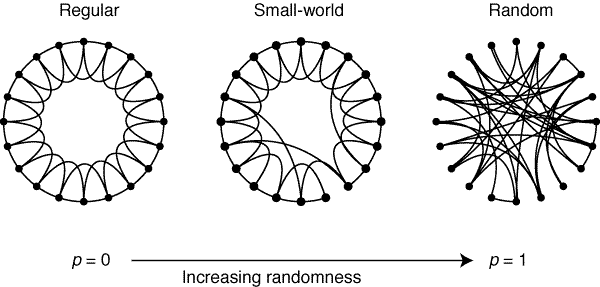
\includegraphics[scale=0.40]{smallworld}
    \caption{Diagram of how networks' properties change as randomness is increased  \cite{smallworld}}
    \label{fig:smallworld}
\end{figure}

As an extension of the random network model, the Watts-Strogatz model describes a network that falls between the orderly characteristics of a lattice and the complex nature of a purely random network.  The Poisson degree distribution of random networks provides an upper bound description of the degree distribution of networks that have the small world property.

%=======================================
\subsection{Scale-Free Networks}

As we saw previously, although random networks predict a degree distribution that follows binomial or Poisson distributions, networks in the real world do no behave in this manner. This led to the development of what are known as scale-free network models which are much better at characterizing the behavior of real network systems. Scale-free models follow what's known as a power law distribution:

\begin{equation}\label{eq:power}
    p_k \approx k^{- \gamma }
\end{equation}


The major differences between random and scale-free models are that random networks fail to capture the effect of hubs and clustering on an entire system.  This is illustrated in Fig. \ref{fig:power} when looking at how a predicted degree distribution of a random network compares to that of an actual network.

\begin{figure}[h]
    \center
    \label{fig:power}
    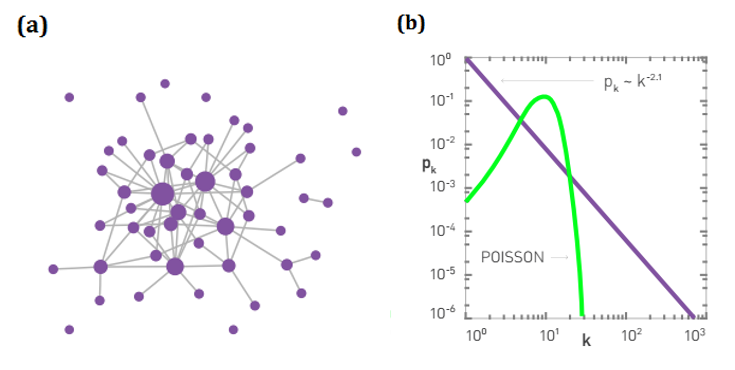
\includegraphics[scale=0.7]{ns-poisson2powerfinal}
    \caption{A scale-free network with $avg(k) = 3$ and $N=50$. The predicted Poisson distribution is plotted in green, the network's actual distribution is plotted in purple. (a) diagram of the network where nodes are sized according to degree, (b) a log-log plot of the network's degree distribution \cite{ns}}
\end{figure}

It is important to understand the implications behind what it means for a network to be ``scale-free.''  Consider the degree $k$ of a randomly selected node.  In random networks, the average degree of this chosen node falls within a range of $avg(k) \pm \sigma _k$.  However, when selecting a node from a scale free network, the range of possible values of the degree of this node is so large that there is no measurable scale.

\begin{figure}
    \centering
    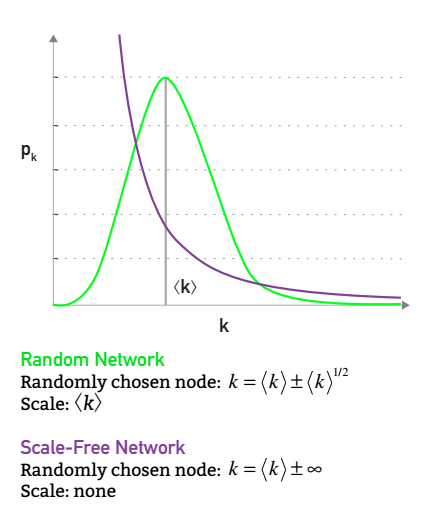
\includegraphics{ns-random2sf}
    \caption{Degree distribution of a random (green) and scale-free network (purple) \cite{ns}}
    \label{fig:rand2sf}
\end{figure}

Consider the $n$th moment of a degree distribution (from statistics).  The first moment is the average degree of a network, and the second moment ($n=2$) is what gives us the variance of the average degree of the network.  As $N \rightarrow \infty$, the second moment of a Poisson distribution is always smaller than than its first.  But in contrast, the second moment of scale-free networks can diverge. (See Fig. \ref{fig:rand2sf})


\section{Conclusion}
We have presented a brief overview of some essential models that have arose from the development of the network science field.  Although the field itself is still relatively new, it has far-reaching applications to a surprisingly diverse range of fields.  

Scale-free models are astoundingly universal. These systems can be found in nature, man-made constructs such as the internet.  Fields such as connectomics in neuroscience aim to study brain networks on micro-, meso-, and macro-scale levels. The rise of social networks like Facebook and Instagram is now heavily studied by advertisers and social engineers alike. Even sometime as simple as optimizing airline routes reveals an underlying scale-free network. (see Fig. \ref{fig:airline}.)

\begin{figure}
    \center
    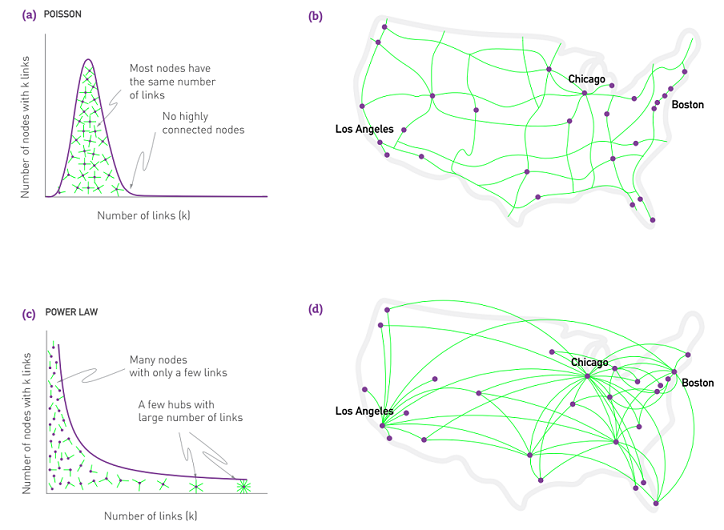
\includegraphics[scale=0.85]{ns-airportmap}
    \caption{A visual map representation of what potential airline routes that follow a Poisson (random network) distribution versus a power law (scale-free network) distribution. \cite{ns}}
    \label{fig:airline}
\end{figure}

It is outside the scope of this paper, but it is worth mentioning that there are many other models and topics not covered here that are relevant to our everyday lives.  For instance, the centrality measurements focus on defining the ``importance'' of nodes based on their degree, weighted degree, and degree of neighboring vertices.  Different algorithms exist to carry out these calculations and each has their own strengths and weaknesses in terms of how accurate, efficient, and useful they are.  Probably the most well-known algortihm is \textit{PageRank}, the trade named algorithm Google created for its web search engine.



\bibliographystyle{unsrt}
\bibliography{references}

\end{document}
